\chapter{Versuch 1: Kapazitätsmessung eines unbekannten Kondensators}

\section{Einleitung}
In diesem Versuch wird die Kapazität eines unbekannten Kondensators
mit Hilfe eines Oszilloskops und eines Funktionsgenerators bestimmt.
Anschließend wird eine Fehlerrechnung durchgeführt.


\section{Vorbereitung}
\subsection{Benötigte Geräte}

Für den Versuch werden folgende Geräte benötigt

\begin{tabular}[h]{c|c}
    Kondensators unbekannter Größe (1nF $\le$ C\textsubscript{x} $\le$ 10nF) \\
    \hline
    Widerstand 4,7 k$\Omega$& \\
    \hline
    Funktionsgenerator & T3AFG80\\
    \hline
    Digital-Multimeter & Fluke TRUE RNS MULTIMETER\\
    \hline
    Oszilloskop & Keysight DSOX1102A
    \label{tab:Versuch 1: Geräte}
\end{tabular}

\subsection{Ziel des Versuchs}
Für einen unbekannten Kondensator in einer BlackBox ist ein Bereich der Kapazität
1nF$\le$C\textsubscript{x}$\le$10nF angegeben. Ziel dieses Versuches ist es, 
die Kapazität des Kondensators genau zu bestimmen und eine Fehlerrechnung durchzuführen.



\section{Versuchsdurchführung}


\subsection{Ladekurve des Kondensators}
Der Kondensator hat eine Ladekurve, die mit der Gleichung 
\[U\textsubscript{C} = U\textsubscript{0} \left(1 - e^{-\frac{t}{\tau}}\right), \tau=RC\]
beschrieben werden kann.\par
Die Ladekurve sieht folgendermaßen aus: 

\begin{figure}[H]
	\centering
	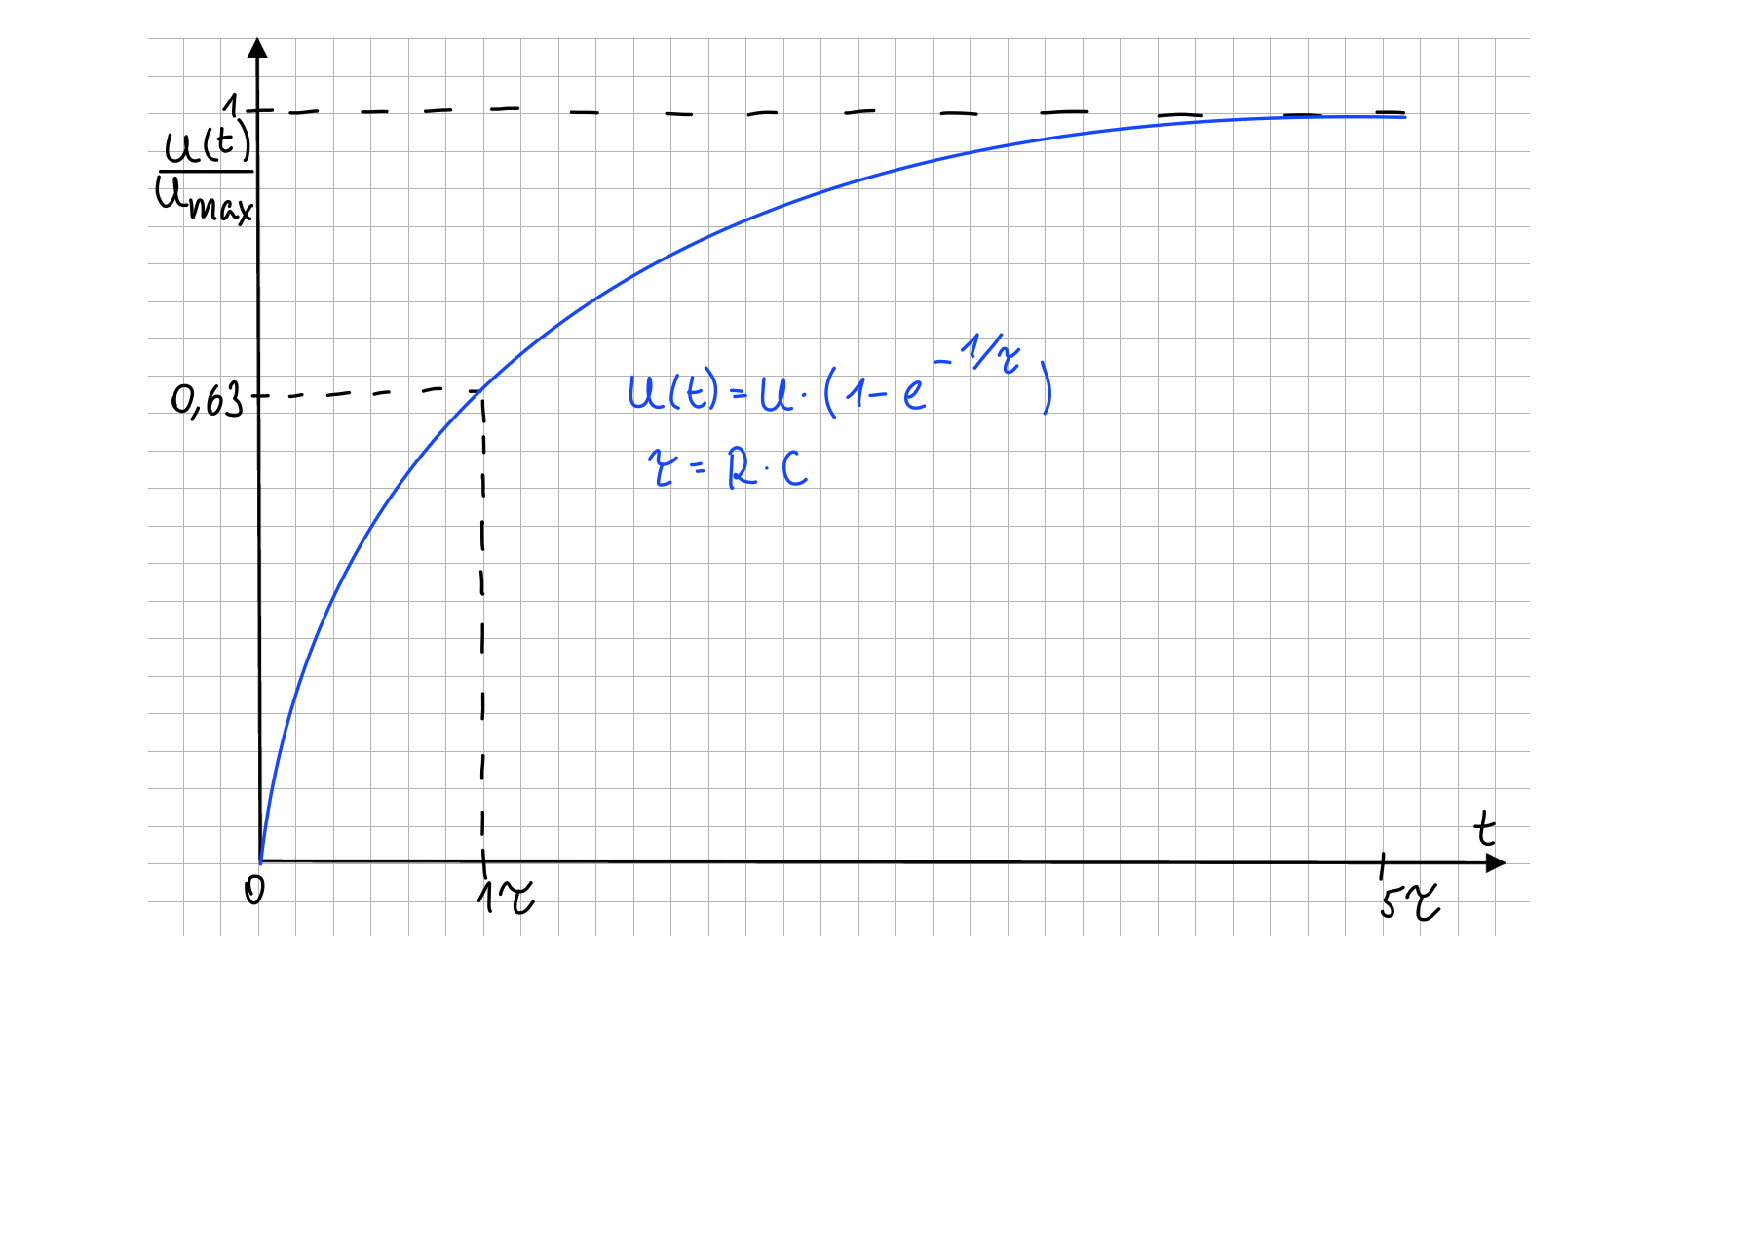
\includegraphics[height=7cm]{images/Versuch1/Ladekurve_zeichnung.pdf} 
	\caption{Ladekurve des Kondensators}
	\label{fig: Ladekurve des Kondensators}
\end{figure}

Nach einem $\tau$ erreicht der Kondensator 62.3\% seiner maximalen Spannung. 

\subsection{Erstellen einer Schaltung}

Man erstellt eine Schaltung, mit der das Lade- und Entladeverhalten des Kondensators
mit dem Oszilloskop beobachtet werden kann. Dafür wird der Frequenzgenerator
durch den Vorwiderstand R\textsubscript{V} mit dem Kondensator verbunden.
Die Messung erfolgt mit dem Oszilloskop parallel zum Kondensator, 
die Masseklemme des Tastkopfs sollte möglichst nah an dem Frequenzgenerator
platziert werden.

Dadurch, dass man den Kondensator direkt mit U\textsubscript{max} aufladen
muss, verwendet man den Rechtecksignal. Die Amplitude des Signals liege 
im Intervall zwischen ca. 3 und 10 Vpp. Man verwendet hier kein Offset.
Resümierend, entsteht hier folgende Schaltung:
\begin{figure}[H]
	\centering
	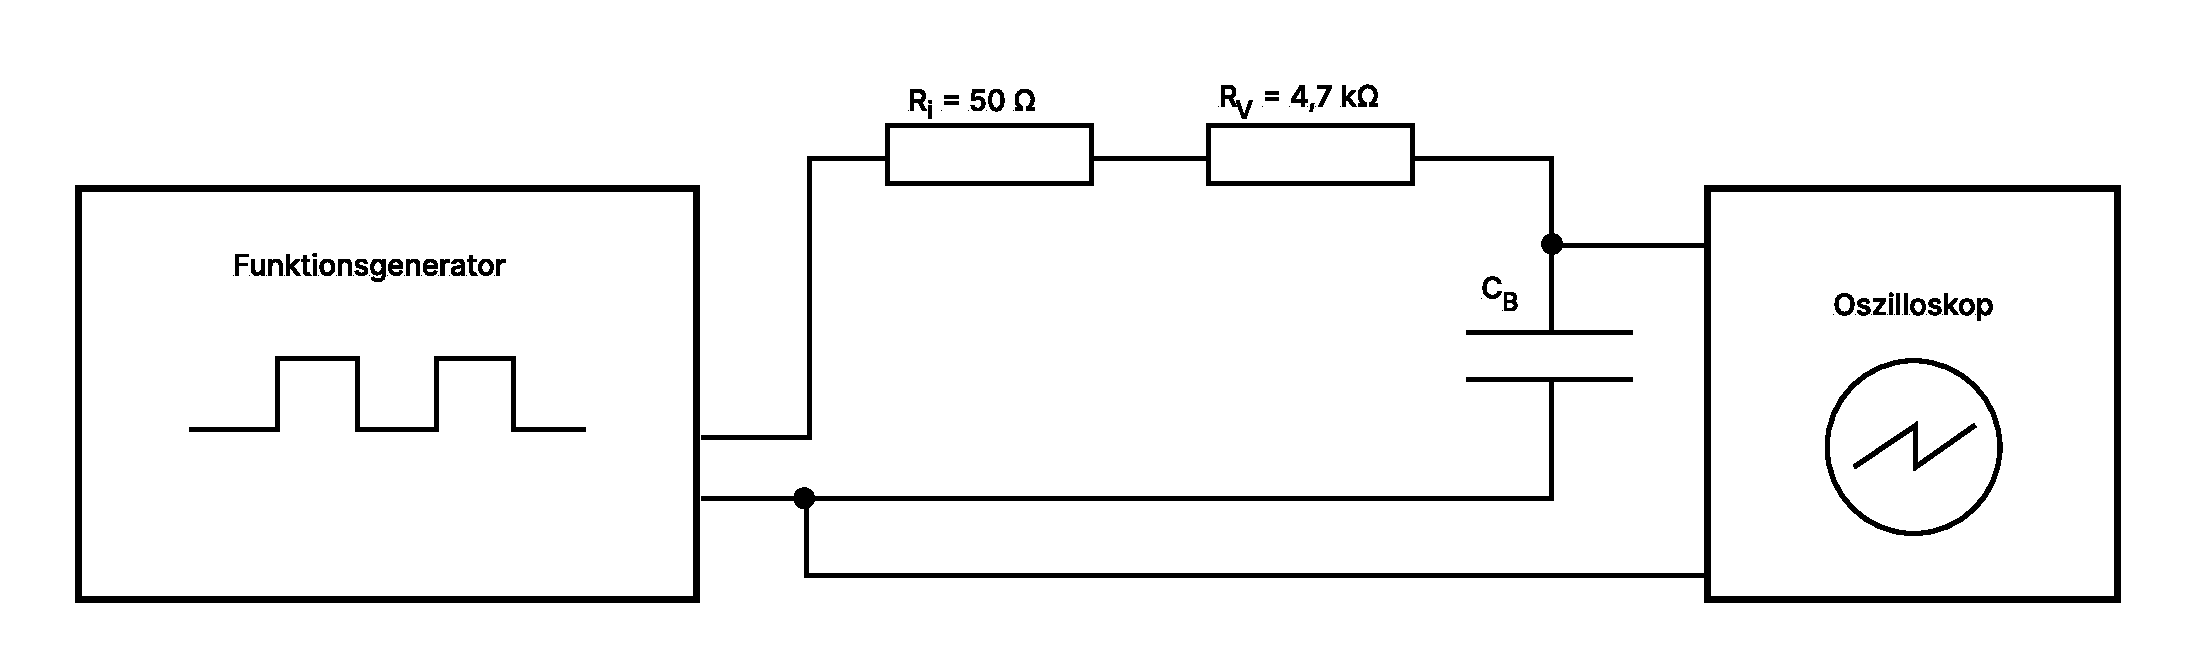
\includegraphics[height=5cm]{images/Versuch1/Schaltbild_versuch1.pdf} 
	\caption{Schaltskizze}
	\label{fig: Schaltskizze}
\end{figure}

Der nahezu vollständie Ladevorgang dauert ca. 5 $\tau$. Basierend darauf kann
man den Intervall für die im Schaltung verwendete Frequenz berechnen:

\[
    f = \frac{1}{5\tau} \hspace{0.5cm} \text{mit} \hspace{0.2cm} \tau = RC
\]

Für C = 1 nF gilt:
\[
    \tau =4700 \Omega*10^{-9}F = 4,7*10^{-6}s
\]

Für C = 10 nF gilt:
\[
    \tau =4700 \Omega * 10*10^{-9}F = 4,7*10^{-5}s
\]

Somit gilt für die Frequenz: \[ f \in I=[4255Hz; 42553Hz] \]

\subsection{Versuchsaufbau und Messung}
Vor der Aufbau wird der im Versuchsberschreibung angegebene Wiederstand 
von 4,7 k$\Omega$ mit dem Digital-Multimeter überprüft. Dieser liegt 
mit 4,583 k$\Omega$ im Toleranzbereich von 5\%. 

Mit dem BlackBox 27 baut man die Schaltung auf. Es resultiert folgende Anordung:
\begin{figure}[H]
	\centering
	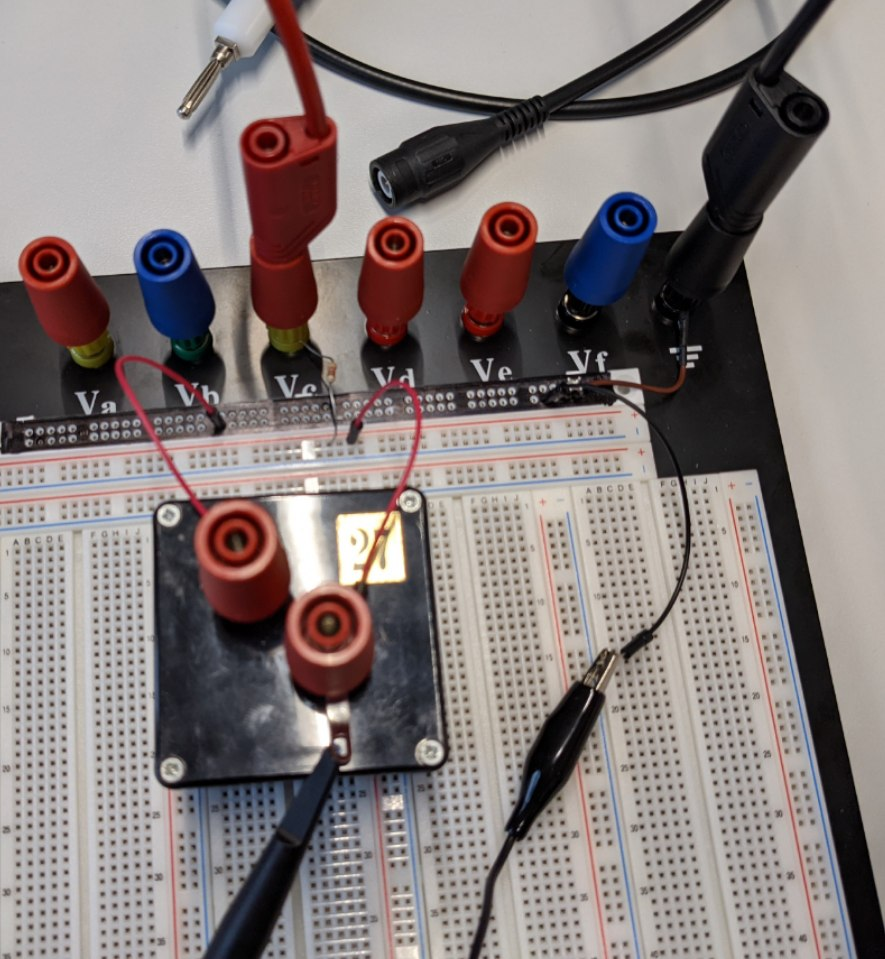
\includegraphics[height=7cm]{images/Versuch1/Versuch1_schaltung_gebaut.jpg} 
	\caption{Schaltung}
	\label{fig: Schaltung}
\end{figure}

In der Anordung wird ein Rechtecksignal mit der Frequenz 10 kHz, 
der Amplitude 6 Vpp, keinem Offset und Duty 50\% verwendet.

Es wird folgende Ladekurve am Oszilloskop beobachtet:
\begin{figure}[H]
	\centering
	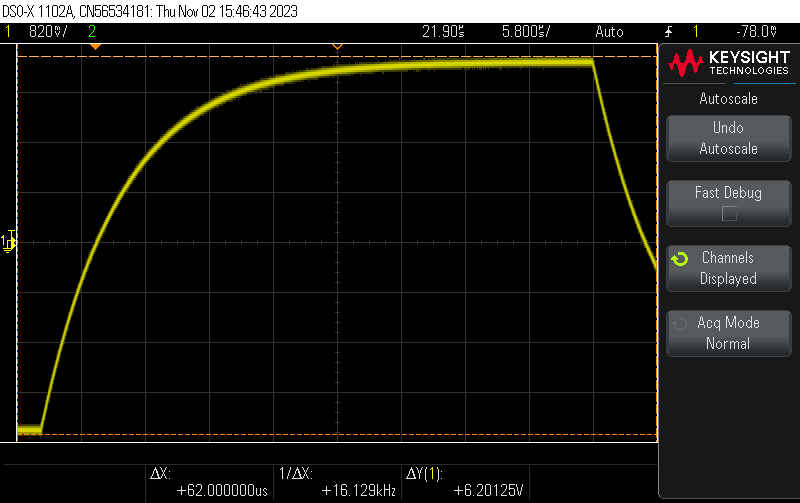
\includegraphics[height=7cm]{images/Versuch1/Ladekurve_voll_6021V.png} 
	\caption{Ladekurve}
	\label{fig: Ladekurve}
\end{figure}

Man beachte, dass trotz angestellter Amplitude in Höhe von
6 Vpp, wird am Oszilloskop 6,21 V Amplitude angezeigt. Mit dieser 
Information wird die Zeitkonstante $\tau$ berechnet. Man kalkuliert
63,2\% von der Amplitude: $6,21V * 0,632 = 3,924V$. Man stellt die 
Y-Cursor auf diese Spannung und misst mit den X-Cursor die Zeit:
\begin{figure}[H]
	\centering
	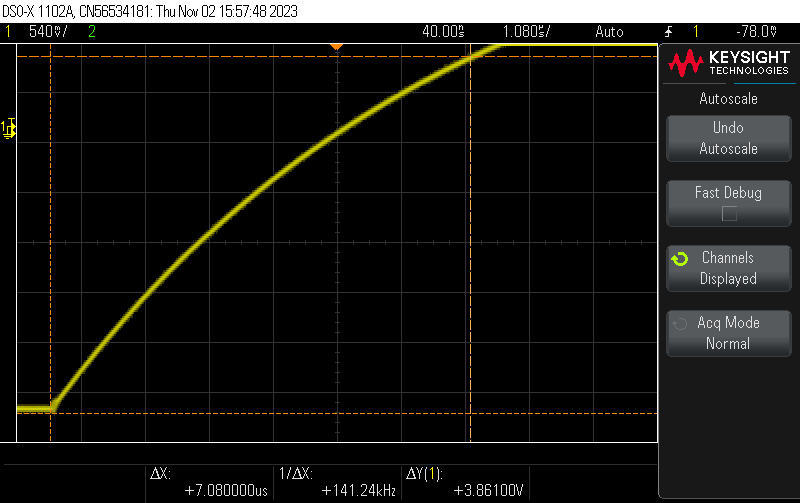
\includegraphics[height=7cm]{images/Versuch1/Zeitmessung.png} 
	\caption{Zeitmessung}
	\label{fig: Zeitmessung}
\end{figure}

Es ergeben sich 7,08 $\mu$s für die Zeitkonstante $\tau$. Die
Einstellungen des Oszilloskops sind folgende:
y: 540 mV/div, x: 1,080 $\mu$s/div.

\subsection{Bestimmung der Kapazität}

Die Kapazität des Kondensators wird mit der Formel für die Zeitkonstante $\tau$
berechnet:
\[
	\tau = R_{ges}C \Leftrightarrow C = \frac{\tau}{R}
\] wobei $R_{ges}$ der Gesamtwiderstand der Schaltung ist
($R_{ges} = R_{i} + R_{V} = 50\Omega + 4,583 k\Omega = 4,633 k\Omega$ ).
Somit gilt für die Kapazität des Kondensators:
\[
	C = \frac{7,08 \mu s}{4,633 k\Omega} = 1,528 nF
\]


\section{Fehlerrechnung}


Fluke 87, Bereich 6k$\Omega$: $\pm[0,02\% + 1 Digit] = \pm[0,02\% \cdot 4583\Omega + 1 Digit] = 0,9166\Omega + 1 Digit = \pm 1,9166\Omega$\par
Full Scale Range: 8 Divs * 540mV = 4,32V\par
Cursorgenauigkeit (dual cursor accuracy): $\pm[3\% + 0,5\% \cdot Full Scale Range] = \pm[3\% + 0,5\% \cdot 4,32V] = \pm 0,0516V = \pm 51,6mV$\par
Screen width: 10 Divs $\cdot$ 1,08 $\mu s$ = 10,8$\mu s$\par
$\Delta$ time accuracy (using cursors): $\pm$[(time base accuracy $\cdot$ reading) $\pm$ (0,0016 $\cdot$ screen width) $\pm$ 200ps] = 
$\pm [85ppm\footnote{Parts per million = $1\cdot10^{-6}$} \cdot 7,08 \mu S + 0,0016 \cdot 10,8 \mu s + 200 ps] = \pm 18,081ns$ \par
x Genauigkeit: $\pm$ 18,081ns\par

\resizebox{\textwidth}{!}{%
	\centering
	\begin{tabular}{c|c|c|c|c|c}
	Fehlerquelle                        					& Einfluss     		& Größe   					& Art         					& Berücksichtigen 							& Relevant            \\ \hline
	R (4,7 k)                          						& DMM (Fluke 87)	& $\pm$ 1,9166$\Omega$ 		& statistisch 					& Fehlerrechnung  							& Ja                  \\ \hline
	\multirow{6}{*}{Oszilloskop	(DSOX1102A) 7 Jahre alt}	& Ri           		& 10 M$\Omega$ $\pm 2\%$ 	& \multirow{2}{*}{systematisch} & \multirow{2}{*}{< 0,5 \textperthousand}   & \multirow{2}{*}{/}  \\ \cline{2-3}
															& Ci           		& 16 pF $\pm 3pF$        	&             					&                 							&                     \\ \cline{2-6} 
															& y            		& $\approx$ 3\%        		& \multirow{2}{*}{statistisch}  & \multirow{2}{*}{Fehlerrechnung}           & \multirow{2}{*}{Ja} \\ \cline{2-3} 
															& x            		& 18,081ns		        	&             					&                							&                     \\ \cline{2-6} 
															& Cursorgenauigkeit & $\pm 51,6mV$        		& statistisch            		& Fehlerrechnung                			& Ja                  \\ \cline{2-6}
															& Time base accuracy& 50ppm+7$\cdot$5ppm = 85ppm& statistisch            		& Fehlerrechnung                			& Ja                  \\ \hline
	\multirow{4}{*}{Funktionsgenerator} 					& Anstiegszeit		& $\approx$ ns       		& systematisch            		& $\approx$ 1 \textperthousand              & /                   \\ \cline{2-6} 
															& Ri           		& 50 $\Omega$        		& systematisch            		& Korrektur                					& Ja                  \\ \cline{2-6} 
															& $\Delta$Ri		& $\approx$ 1\%        		& statistisch            		& $\pm 0,5 \Omega$                			& /                   \\ \cline{2-6} 
															& Amplitude/Offset	& Relativmessung!        	& Relativmessung!             	& /                							& /                   \\ \hline
	Kabel und Steckverbindung           					& Widerstand   		& $\le$ 20m$\Omega$	        & systematisch            		& /                							& /              
	\label{tab: Fehlerrechnung}

\end{tabular}%
}

$\Delta \tau_u$: \\
Für die Ladekurve gilt: $u(t) = U_0 \cdot (1 - e^{-\frac{t}{\tau}})$\\
Dann gilt für die Steigung: $\frac{\partial U}{\partial t} =\frac{U_0}{\tau} \cdot e^{-\frac{t}{\tau}}$, t = $\tau$ = $\frac{U_0}{e\tau} = \frac{6,21V}{e\cdot7,08\mu s} = 322,67\frac{V}{ms}$\\
Somit ist der Beitrag zur horizontalen Messungenaugikeit: $\Delta \tau_u = \frac{51,6mV}{322,67\frac{V}{ms}} = 159,91 ns$\\

Daraus folgt: $\Delta t = \pm (159,91 + 18,081)ns = \pm 177,991 ns$

Messergebnis: $\tau = (7,08 \pm 0,177991) \mu s = 7,08 \mu s \pm 2,51\%$\\

Mit dieser Information kann jetzt maximaler und wahrscheinlicher Fehler der Kapazitätsmessung berechnet werden:\\
Maximaler Fehler:\\ 
Absolut: 
\[
	\Delta C_{1} = |\frac{1}{R} \cdot \Delta \tau| + |- \frac{\tau}{R^2} \cdot \Delta R| = 
	(\frac{1}{4633 \Omega} \cdot 177,91 ns) + (\frac{7,08 \mu s}{(4633 \Omega)^2} \cdot 1,9166 \Omega)
	= 39,032 pF
\]\\
Relativ: 
\[
	\Delta C_{1} = \frac{\Delta C_{1}}{C_{1}} = \frac{39,032 pF}{1,528 nF} = 2,55\%
\]

Wahrscheinlicher Fehler:\\
Absolut: 
\[
	\Delta C_{2} = \sqrt{(\frac{1}{R} \cdot \Delta \tau)^2 + (- \frac{\tau}{R^2} \cdot \Delta R)^2} =
\sqrt{(\frac{1}{4633 \Omega} \cdot 177,91 ns)^2 + (- \frac{7,08 \mu s}{(4633 \Omega)^2} \cdot 1,9166 \Omega)^2}
= 38,4 pF
\]\\
Relativ: 
\[
	\Delta C_{2} = \frac{\Delta C_{2}}{C_{1}} = \frac{38,4 pF}{1,528 nF} = 2,51\%
\]\\


\section{Zusatzfragen}

Durch das BNC Kabel und die Steckverbindung entsteht ein zusätzlicher 
Widerstand von ca. 50 $\Omega$. Dieser Widerstand kann in der Fehlerrechnung
kompensiert werden, indem man den Widerstand in der Schaltung um 50 $\Omega$
kleiner auslegt.

Wenn der Wert des Vorwiderstandes nicht gemessen wäre, sondern mit dem
Nominalwert und Toleranz gerechnet werden würde, dann würde dies einen
Einfluss auf die Kapazitätsmessung haben. Man rechne mit dem Nominalwert
des Widerstandes und der Toleranz von 5\%:

\[
	R_{V} = 4,7 k\Omega \pm 5\% = 4,7 k\Omega \pm 235 \Omega
\]

Dieser Betrag ist deutlich größer als in der Rechnung.
Dadurch erhöhrt sich der Gesamtwiderstand der Schaltung und somit
auch der Fehler der Kapazitätsmessung:

\[
	\Delta C_{1} = (\frac{1}{4700 \Omega} \cdot 177,91 ns) + (\frac{7,08 \mu s}{(4700 \Omega)^2} \cdot 235 \Omega)
	= 113,17 pF
\]

\[
	\Delta C_{2} = \sqrt{(\frac{1}{R} \cdot \Delta \tau)^2 + (- \frac{\tau}{R^2} \cdot \Delta R)^2} =
	\sqrt{(\frac{1}{4700 \Omega} \cdot 177,91 ns)^2 + (- \frac{7,08 \mu s}{(4700 \Omega)^2} \cdot 235 \Omega)^2}
	= 84,29 pF
\]\\

Man erkennt, dass der Fehler der Kapazitätsmessung deutlich größer ist,
denn die Toleranzangaben des Widerstandes viel größer sind als der
eigentliche Fehler des Widerstandes. 